% Chapter 2
%
\chapter{Technology and Basic Principles} % Main chapter title
\label{Chapter2} % For referencing the chapter elsewhere, use \ref{Chapter2} 
%
%2. Technology and basic principles
    %
    %Public Key Cryptography
        
        %Key management

        %Certificates
        %\label{sec:cert} %Discussion of what data certificates usually contain

        %\label{sec:pgp_enc} %Demmonstration/Example of PGP encryption

    %Web of Trust
        %Overview

        %Ceritifcates

        %Certificate sharing

        %Sylbil attack
        %\label{sec:trust_syl} %Sylbil attack theory

    %WebRTC
    %\label{sec:webrtc}
        
        %Connection setuo
            %ICE, STUN \& TURN
            %\label{sec:webrtc_icetri} % WebRTC ICE trickling
            %SDP and DTLS-SCTP
            %Offer and Answer
            %\label{sec:webrtc_off} 

        %Signaling server

    %WS
    %\label{sec:ws}
    
%
% THIS SHOULD GO THROUGH THE TECHNOLOGY OBJECTIVELY AND HOW IT WORKS!
%
This chapter will go over the technologies proposed and used in SendIt and give an introduction to their functionality, as well as the reasons for choosing that technology. It will give a basic understanding of the technology, which the rest of the thesis is built upon.
%
\section{Cryptography}
\label{sec:pkc}
%
    %TODO
    %Key pairs
    The encryption and authentication scheme used in SendIt is based on public key cryptography and symmetric cryptography. Public key cryptography is a technology that creates a public and a private key pair. The public key is used for encryption. The encrypted data can \emph{only be decrypted by the corresponding private key}. The inverse is also true. Anything encrypted with the private key, can be decrypted by the public key. The common usage is to spread the public key around, hence the name public. The private key (also called secret key) is kept safe, and only the identity that is the owner of the key pair should have access to it \cite{trcekManagingInformationSystems2006}.

    In contrast, symmetric cryptography utilizes the same key for encryption and decryption. The advantage of symmetric cryptography is that it can encrypt larger amounts of data. The disadvantage is that anyone with the key, can read any message. Symmetric keys usually also needs a value called IV (\emph{Initialization Vector}), that is used to randomize the encrypted values. It allows for two identical messages to have different ciphers. There are two forms of IV schemes. One is using completely random number(s) each time. This is called a randomized scheme. The other scheme is called stateful, and requires each IV to be unique \cite{bellareIntroductionModernCryptography2005}.

    SendIt uses public key cryptography to exchange encrypted messages that only the person having the correct key can decrypt. This is the same principles as used in Public Key Infrastructure. The difference lies in that PKI relies on a central authority for signing and verifying the keys used, in the form of certificates. SendIt tries to avoid any central form of governance, and as such implements the web of trust model instead, to avoid this central management. This is discussed more in \Cref{sec:trustmodel}.

    \subsection{Key management}
    This means that the keys have to be the same every time, which requires each user to store their keys for later. This should be done with some consideration, since a stolen private key means anyone can now take your identity and successfully authenticate as you. As such the need for secure storage arises. This can be solved by encrypting the keys with a password, then storing them on the local machine. Only when a key is in use, will it be read and decrypted. This decreases the chance of the key being stolen, since it minimizes the attack surface by only having the key available when it is in use.

    When storing keys it is necessary to keep more information than just the key. For example it is also necessary to know who it belongs to. For the proposed system, information relevant to the trust-level of each key also needs to stored. The easiest way to do this, is to store the certificate of each key with the key. That means the trust for a key will have to be re-calculated every time it is loaded. This is costly when it comes to computational resources, but allows the system to re-calculate the trust  in a key before each use. This gives a flexible and up-to-date environment where trust is evaluated similar to in the real world.

    \subsection{Certificates}
    \label{sec:cert}
    %
    SendIt also proposes to use digital certificates, like the ones used in the web of trust model \cite{ar_pgp}. Certificates traditionally contain lots of information. The certificate is then signed by any number of “introducers”, by encrypting it using their private key. An introducer is an identity who trusts another identity and vouches for the legitimacy of that identity \cite{ar_pgp}.
    
    Certificates used in PKI are required to contain enough information to provide a third party with the subject's public key. Usually certificates used in PKI contain more data than required. The minimum require data can be summed up in four points \cite{vaccaPublicKeyInfrastructure2004}:\\
    \begin{itemize}
        \item CA identification information
        \item Subject identification information
        \item Subject public key
        \item Validity (time)
    \end{itemize}
    More information on introducers and certificates can be found in \Cref{sec:trustmodel}.

    \subsection{Authentication}
    \label{sec:pgp_enc}
    The last part of the puzzle is: how can a user be authenticated based on this information? There are many different schemes but SendIt focuses on the one suggested by PGP for securely exchanging messages \cite{b_pgp}. The system is based on public key encryption. It also uses a session key, which is a random, one time generated symmetric key. The system guarantees the authenticity, confidentiality and integrity of the data. Encryption and decryption using the PGP system is shown in \Cref{fig:enc} and \Cref{fig:decr}.

    The way PGP works is by first generating a symmetric key and encrypting the data to be transferred with this symmetric key. This results in a cipher. Let us call this \emph{Cipher 1}. Then the symmetric key is encrypted with the recipients public key. This also results in a cipher. Let us call this \emph{Cipher 2}. The data transferred to the recipient is Cipher 1 and Cipher 2.

    The recipient then retrieves the symmetric key, by decrypting \emph{Cipher 2}, using their private key. Then, using the retrieved symmetric key, \emph{Cipher 1} is decrypted and the original data is available.

    This solution is made with a one-directional exchange of data in mind. We will be using this system to authenticate both endpoints, which means we will have bi-directional communication. The way to solve this issue, is by taking advantage of the way symmetric keys encrypt data. The initial exchange from Sender to Receiver gives proof to the Sender that the recipient is as intended. This is not the case if we re-use the same IV for the reply back. As such, it should be changed.

    Usually the IV is shared in cleartext, since knowledge of the key is required to decrypt it, so it is not sensitive data. In SendIt we encrypt the IV used in the reply with the recipients public key. That means that in order to be able to access the data, the private key is needed, and as such, the Sender is also authenticated. This solves the issues of mutual, bi-directional authentication.

%
\section{Web of trust}
\label{sec:trustmodel}
%
    This section is a suggestion and evaluation of the system only. This has not been implemented in SendIt due to time constraints, but is considered a part of the design.

    \subsection{Overview}
    The model suggested is based on the web of trust model. The web of trust model says that trust should be split in to two groups: \textbf{Trustworthiness of public-key certificate} - \emph{How willing are you to trust this key pair when it is being used to communicate?} and \textbf{Trustworthiness of introducer} - \emph{How willing are you to trust this key pair when it is being used to introduce another key?}.

    It also suggest that the trust level given to a key should be based on points given to a certificate, based on the sum of introducer's and their respective trust level. There is no concrete policy or algorithm suggested for evaluating which level of trust is assigned. The paper does define levels of trust, but they are different for the two groups mentioned above. 

    There is also no recommendation of which trust level should be considered safe or unsafe. This is left up to each individual user \cite{ar_pgp}. There exist many ways to rate and evaluate trust. For this system, a simple point-based system is likely to be the best fit. The web of trust model has also been recommended by other researchers, albeit for a more traditional WebRTC authentication system \cite{ar_whois}. For a look in to more options, J\o sang et al. 2007 \cite{a_trustserv} gives a good overview over possible alternatives.

    \subsection{Certificates}
    %
    The way one infers, evaluates and determines trust is by using certificates. The trust is evaluated based on interactions with others and the interactions between trusted introducers and others. This means that information from identities one does not trust will be disregarded (their introductions mean nothing), while still valuing and receiving updated information from identities one does trust.In other words, many untrusted identities introducing someone does not hold any value, while introductions from a few trusted identities has a significant impact on the trust level assigned to a certificate.

    \subsection{Certificate-sharing}
    The exchange of keys and the trust each identity assigns these keys are central to the web of trust model, as described above (\Cref{sec:trustmodel}). Since the connection used for communication is already secure and each party authenticated, this data can be transferred without additional encryption. This section will describe how this is intended to be implemented in SendIt. This is included as part of this Chapter since it has not been implemented in practice.
    %
        \subsubsection*{Request certificates:}
        SendIt will have an automated, bi-directional sharing of certificates, that happens on every exchange. This sharing will be part of the file transfer-protocol and will happen after the file-transfer has completed (before terminating the connection). This automatic sharing will abstract the system away from the user, to make the system easy to use and understand, while still updating the trust-level for different identities according to recent changes in the system. The choice to make this part mandatory also allows for the system to avoid being biased by only receiving updates from certain identities.
        %
        \subsubsection*{Evaluate certificates:}
        While exchanging certificates with all communication-partners is important to avoid biases, it is also important to let the user influence and differentiate the level of trust given to each partner. This is where settings and evaluation comes in to play. Each user can change the level of trust in each partner manually, based on his own preferences.

        As an extension of the trust given to each partner, the information they share, is also evaluated based on how trusted the partner is. The trust evaluation of each key, and by extension each identity, will vary depending on user settings and preferences. It will however always follow the scheme as described above. The effect of this evaluation will result in a corresponding trust-level associated with the identity. Identities that have too low a trust level to be used can either raise a untrusted-user warning before communication occurs, or a connection terminated message, depending on the users settings. These keys will still be stored in the users key-chain and stay available for future evaluation, even if their current level of trust is low.

    \subsection{Sylbil attack}
    \label{sec:trust_syl}
    A common attack in decentralized reputation systems is the Sybil attack. It is an attack that takes advantage of the fact that the system can be manipulated by having a large number of identities share the same, false information to innocent identities. In SendIts case, that a certain key pair belongs to a certain identity, while in fact it does not. Through sheer numbers, the attack manipulates identities in the system to believe that the attacker should be the trusted identity, not the original identity. This misleads users to connect to the wrong identity, which makes them vulnerable to attacks. It can also lead to being unable to connect to the legitimate identity, since all traffic for that identity is instead routed to the attacker \cite{lncs_sybil}.

%
\section{WebRTC}
\label{sec:webrtc}
%
    WebRTC is a fairly new technology developed for real-time communication between web entities. It focuses on allowing video, audio and data transfers over P2P, through an easy to use API. It does this without the need to install plugins or having to download native applications, since it is already implemented in most of today's popular browsers. 

    %Connection setup
    \subsection{Connection setup}
    \label{sec:conn_setup}
    %
    To set up a connection using WebRTC, there are different variables one has to take in to account. First, what are the network conditions for each endpoint? To be able to create a connection, we need to find a way to address each endpoint directly. To do this WebRTC utilizes STUN \cite{ar_stun} and/or TURN \cite{ar_turn}, and ICE \cite{ar_ice}. 
    %
    \subsubsection*{ICE, STUN \& TURN}
    \label{sec:webrtc_icetri}
    %
    The ICE-protocol works by trying to connect directly to the endpoint. If an endpoint is behind symmetrical NAT, however, a TURN server is required. A TURN-server acts as a relay-server that both endpoints connect to, and there is no longer a direct P2P-connection. Instead each endpoint is connected to a server by a P2P-connection, and the server forwards information to the other end. It is the ICE-protocol that manages these issues and tries to find the best possible connection \cite{ar_webrtc_sign}.

    %Add more detail on ICE trickling! Picture? TODO
    ICE is a protocol for NAT-traversal used in offer/answer protocols. In regular WebRTC-applications, something called ICE-trickling is used. This is because generating the offer and the answer is quick, but gathering ICE candidates takes time. This allows the setup of the channel to happen first, then ICE-candidates to be shared afterwards \cite{ar_ice_trickle}. In SendIt this functionality is utilized in the ACS mode.

    In serverless mode all the information is gathered, then attached to the offer/answer and then shared. ICE is used to be able to address and reach computers behind NAT \cite{ar_ice}. The easiest way to describe the whole process is to imagine ICE as the decision maker, utilizing STUN and TURN to find information about the endpoint. Once all the information from STUN and TURN is gathered, ICE prioritizes the information, and shares it as separate possible ways to connect to the endpoint. These connection alternatives are called ICE candidates.
    %
    \subsubsection*{SDP and DTLS-SCTP}
    %
    SDP stands for Session Description Protocol, and is a format for session descriptions. This is a protocol for formatting data, for example discovered through the ICE-protocol, to be shared with the other endpoint \cite{ar_sdp}. For the serverless mode, it is up to the users how they share the offer and answer, and as such it does not use a transfer-protocol. In the ACS mode, secure WebSockets are used for sharing the information.

    The WebRTC datachannels used for direct communication uses DTLS-SCTP as their transport-protocol \cite{ar_webrtc_dc}.
    %
    \begin{quotation}
        \enquote{DTLS itself is modelled upon the stream-orientated TLS, a protocol which offers full encryption with asymmetric cryptography methods, data authentication, and message authentication \cite{StudyWebRTCSecurity}.}
    \end{quotation}
    %
    In other words, the communication is securely transported between the endpoints, once the connection setup is done.

    %WRITE XEXPLICITLY! TODO
    The encapsulation of SCTP over DTLS, ICE- and SDP-protocols are complex. For those unfamiliar with the technology, an in depth explanation is given in Holmberg, H.-C. (2015)\cite{url_webrtc_data}. In summary: each endpoint gathers the necessary connection data and then formats it according to the SDP-protocol, for session-negotiation and initiation. Then the datachannel is created and the connection is made.
    %
    \subsubsection*{Offer and Answer}
    \label{sec:webrtc_off}
    %
    Following is how the relevant RFC describes how endpoint guarantee is done:
    %
    \begin{quotation}
        \enquote{A certificate fingerprint is a secure one-way hash of the DER (distinguished encoding rules) form of the certificate. If the X.509 certificate presented for the TLS connection matches the fingerprint presented in the SDP, the endpoint can be confident that the author of the SDP is indeed the initiator of the connection \cite{ar_tls_sdp}.}
    \end{quotation}
    %
    This explanation can be a little hard to understand, so let us break it down. Both the offer and the answer generated by the WebRTC API has a fingerprint of a certificate attached. The endpoint generates a X.509 certificate and a corresponding private key. By matching the fingerprint received during signaling, with the certificate used during the setup of the DTLS-SCTP connection, one can be certain that the endpoint is the same. This is illustrated in \Cref{fig:DTLS_setup}.
    %
    \begin{figure}[t]
      \centering
      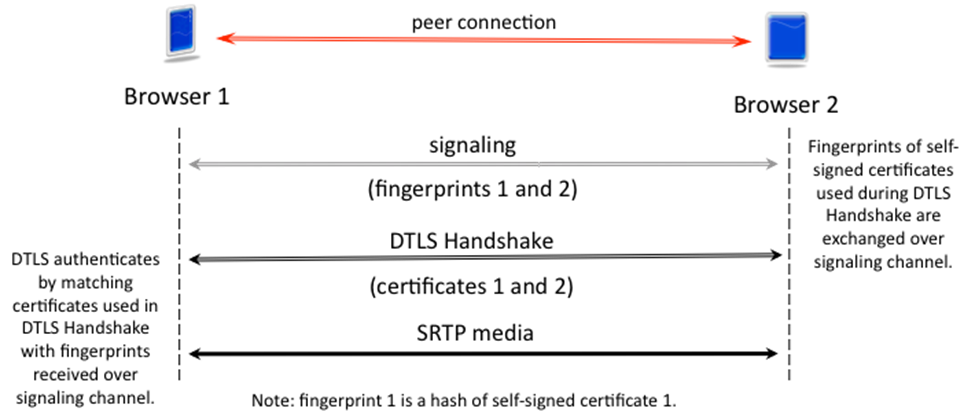
\includegraphics[width=\textwidth]{Figures/DTLS_Exchange}
      \decoRule
      \caption[DTLS setup]{Illustration shows and describes how DTLS is setup between two endpoints. The final channel in the illustration is of the type SRTP, but the same procedure is true for SCTP \cite{WebRTCManMiddle2015}}
      \label{fig:DTLS_setup}
    \end{figure}
    %
    \subsection{Signaling server}
    \label{sec:sign_serv}
    %
    In the usual use-case of WebRTC, a signaling-server is used to share SDP offers and answers, as well as continuously sharing ICE-candidates. This separate channel allows for re-negotiation of communication, if the connection breaks down. An offer is the exchange of SDP information from the sender, to the receiver. An answer is the exchange of SDP information from the receiver, to the sender.

    There is several reasons for the usage of a signaling-server. One is the ability to reconnect in the event of a failure in the established connection. Another is that it allows the offer and answer to not be created until both endpoints are online, then immediately created and shared. This is the case when using ACS. When using serverless mode, however, this is not the case. This means it is affected by the fact that network conditions can change rapidly and as such ICE-candidates may no longer be viable, leaving endpoints with no way to make a connection or renegotiating the connection. For more information on the lifetime of the exchange, see \Cref{Chapter5}.

    Another use of the signaling-server is that it allows for encrypted communication between the parties, via the server. As long as you trust the signaling-server, your communication is confidential. This is important in regards to the exchange of the offer/answer, as they contain information that allows a secure connection to be set up, as described in the section above.

    In the Serverless mode we do not have a secure channel over which we exchange the offer/answer. That means it would be vulnerable to a MitM-attack. To combat this the offer and answer will be encrypted by each endpoints public key, on all connections after the first (See \Cref{fig:enc} for illustration). With this protection in place an attacker can not get a hold of the offer/answer, without stealing the private key that can decrypt the cipher.

%
\section{WebSockets}
\label{sec:ws}
%
To understand why WebSockets are necessary, let us first examine how normal communication between client and server is done. The client sends a request and the server sends a response. If the data contained in the response is time critical, it will in many cases already be outdated by the time it is rendered by the client. A manual way to combat this is to refresh the page. A more elegant way is the use of polling. Polling is a regularly timed, synchronous call the client makes to the server, to look for new information. This works well if you can predict when new data will be available. The problem is that this is often not the case. There are other alternatives as well, for example long polling or streaming, but they all come with certain issues regarding real-time, two-way communication. Especially latency and overhead are big issues.

This is where WebSockets come in to play. WebSockets offer real-time, duplex, bi-directional connection. It makes communication between a client and server easier and faster. It also supports real-time communication, which is an added bonus. WebSockets are commonly used in a lot of real-time applications in today's online environment. From transferring game data to simple chat applications. It is also commonly used for signaling in WebRTC applications. This is also how it is used in SendIt, specifically in the ACS mode.

Another great thing about WebSockets, is that it supports the traditional use of TLS. This means that the WebSocket protocol can use the same security mechanisms as traditional HTTPS traffic. This makes it easy to protect the confidentiality, integrity, and availability of your network communications. Finally, all modern browsers have native support for the WebSocket protocol and as such it is incredibly easy to deploy \cite{wangDefinitiveGuideHTML52013}. For these reasons, the WebSocket protocol was chosen to take care of the communication between endpoints and the Server, required by the ACS mode.

